\RequirePackage{currfile} 

\documentclass[aspectratio=169]{beamer}

%%%%%%%%%%%%%%%%%%%%%%%%%%%%%%%%%%%%%%%%%
% Beamer Presentation
% LaTeX Template
% Version 1.0 (10/11/12)
%
% This template has been downloaded from:
% http://www.LaTeXTemplates.com
%
% License:
% CC BY-NC-SA 3.0 (http://creativecommons.org/licenses/by-nc-sa/3.0/)
%
%%%%%%%%%%%%%%%%%%%%%%%%%%%%%%%%%%%%%%%%%

%----------------------------------------------------------------------------------------
%	PACKAGES AND THEMES
%----------------------------------------------------------------------------------------




\mode<presentation> {

% The Beamer class comes with a number of default slide themes
% which change the colors and layouts of slides. Below this is a list
% of all the themes, uncomment each in turn to see what they look like.

%\usetheme{default}
%\usetheme{AnnArbor}
% \usetheme{Antibes}
% \usetheme{Bergen}
%\usetheme{Berkeley}
\usetheme{Berlin}
%\usetheme{Boadilla}
% \usetheme{CambridgeUS}
%\usetheme{Copenhagen}
%\usetheme{Darmstadt}
%\usetheme{Dresden}
%\usetheme{Frankfurt}
%\usetheme{Goettingen}
%\usetheme{Hannover}
%\usetheme{Ilmenau}
%\usetheme{JuanLesPins}
%\usetheme{Luebeck}
%\usetheme{Madrid}		
%\usetheme{Malmoe}
%\usetheme{Marburg}
%\usetheme{Montpellier}
%\usetheme{PaloAlto}
%\usetheme{Pittsburgh}
%\usetheme{Rochester}
%\usetheme{Singapore}
%\usetheme{Szeged}
% \usetheme{Warsaw}

% As well as themes, the Beamer class has a number of color themes
% for any slide theme. Uncomment each of these in turn to see how it
% changes the colors of your current slide theme.

% \usecolortheme{albatross}
% \usecolortheme{beaver}
% \usecolortheme{beetle}
% \usecolortheme{crane}
% \usecolortheme{dolphin}
% \usecolortheme{dove}
% \usecolortheme{fly}
\usecolortheme{lily}
% \usecolortheme{orchid}
% \usecolortheme{rose}
% \usecolortheme{seagull}
% \usecolortheme{seahorse}
% \usecolortheme{whale}
% \usecolortheme{wolverine}

%\setbeamertemplate{footline} % To remove the footer line in all slides uncomment this line
%\setbeamertemplate{footline}[frame number] % To replace the footer line in all slides with a simple slide count uncomment this line

%\setbeamertemplate{navigation symbols}{} % To remove the navigation symbols from the bottom of all slides uncomment this line

% \setbeamercovered{transparent} % Fait apparaître les animations en grisé (utile pour la conception, mais peut être commenté lors de la remise du document final)

% Pour utiliser une police à empattements partout
\renewcommand{\familydefault}{\sfdefault}

% Pour rajouter la numérotation des frames dans les pieds de page
\newcommand*\oldmacro{}%
\let\oldmacro\insertshorttitle%
\renewcommand*\insertshorttitle{%
  \oldmacro\hfill%
  \insertframenumber\,/\,\inserttotalframenumber}

}

\usepackage{graphicx} % Allows including images
\usepackage{booktabs} % Allows the use of \toprule, \midrule and \bottomrule in tables

\setbeamertemplate{caption}[numbered]
\newcommand\subheading[1]{%
  {\Large\bfseries#1}\par\smallskip}
\usepackage{natbib}        
\usepackage{url}           
% \usepackage[T1]{fontenc}   
% \usepackage[utf8]{inputenc}
% \usepackage[english]{babel}
\usepackage[utf8]{vietnam}
\usepackage{numprint}      

\usepackage{amsmath}       
\usepackage{mathrsfs}      
\usepackage{amssymb}       
\usepackage{amsfonts} 

\usepackage{cancel}


\usepackage{minted}
\usemintedstyle{friendly}

\usepackage{graphicx}
\usepackage{wrapfig}  

\usepackage{tikz}     

% \usepackage[framemethod=TikZ]{mdframed}
% \usepackage[T1]{fontenc}
% Ce fichier contient toutes les macros que vous pouvez avoir envie de définir 
% si vous les utilisez plusieurs fois dans le document.

\PassOptionsToPackage{svgnames}{color}

% Un environnement pour bien présenter le code informatique
\newenvironment{code}{%
\begin{mdframed}[linecolor=green,innerrightmargin=30pt,innerleftmargin=30pt,
backgroundcolor=black!5,
skipabove=10pt,skipbelow=10pt,roundcorner=5pt,
splitbottomskip=6pt,splittopskip=12pt]
}{%
\end{mdframed}
}

% Un raccourci pour composer les unités correctement (en droit)
% Exemple: $v = 10\U{m.s^{-1}}$
\newcommand{\U}[1]{~\mathrm{#1}}

% Les guillemets \ofg{par exemple}
\newcommand{\ofg}[1]{\og{}#1\fg{}}

% Le d des dérivées doit être droit: \frac{\dd x}{\dd t}
\newcommand{\dd}{\text{d}}

% La dérivée temporelle, tellement courante en physique, avec les d droits
\newcommand{\ddt}[1]{\frac{\dd #1}{\dd t}}

% Des parenthèses, crochets et accolades qui s'adaptent automatiquement à la 
% taille de ce qu'il y a dedans
\newcommand{\pa}[1]{\left(#1\right)}
\newcommand{\pac}[1]{\left[#1\right]}
\newcommand{\paa}[1]{\left\{#1\right\}}

% Un raccourci pour écrire une constante
\newcommand{\cte}{\text{C}^{\text{te}}}

% Pour faire des indices en mode texte (comme les énergie potentielles)
\newcommand{\e}[1]{_{\text{#1}}}

% Le produit vectoriel a un nom bizarre:
\newcommand{\vectoriel}{\wedge}


\title[Sinh biểu cảm khuôn mặt dựa trên phù hợp giọng nói]{\textbf{SINH BIỂU CẢM KHUÔN MẶT DỰA TRÊN PHÙ HỢP GIỌNG NÓI}}

\author{Trần Hoàng Tuấn\inst{1}, Lê Thành Sách\inst{2}}

\institute[HCMUT]{
\inst{1}%
Học viên thực hiện\\
Khoa học máy tính, đại học Bách Khoa thành phố Hồ Chí Minh
\and
\inst{2}%
Tiến sĩ hướng dẫn khoa học\\
Khoa học máy tính, đại học Bách Khoa thành phố Hồ Chí Minh }
\date{Bảo vệ đề cương luận văn, 01/2021} 

\begin{document}
\begin{frame}
\titlepage 
\end{frame}
\frame{\tableofcontents}

\section{Giới thiệu}\label{sec:intro}
\frame{\tableofcontents[currentsection]}
\begin{frame}{Giới thiệu}

\begin{itemize}
    \item Là một bài toán tạo sinh dữ liệu dạng hình ảnh dựa trên các dạng dữ liệu khác.
    \item Cho trước một vài dữ liệu về gương mặt của một người bất kỳ \textit{(hình ảnh, video ngắn)} và môt đoạn tiếng nói bất kỳ. Tạo sinh hình ảnh người đó đang nói đoạn tiếng nói đã cho một cách chân thực.
\begin{figure}[H]
    \centering
    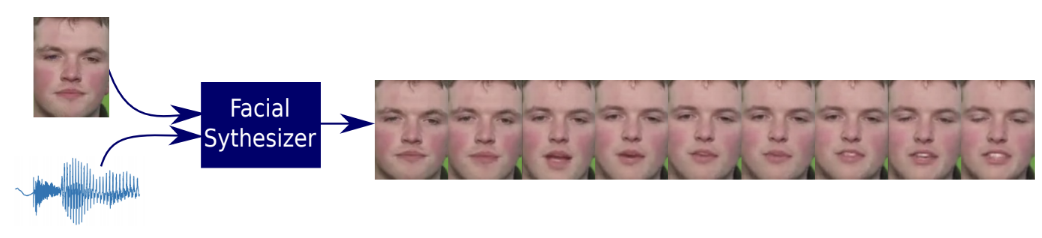
\includegraphics[width=13cm]{images/intro.png}
    \caption{Ví dụ về mô hình tạo sinh khuôn mặt}
    \label{fig:example}
\end{figure}
\end{itemize}
\end{frame}

\section{Mục tiêu, giới hạn và đối tượng của nghiên cứu}\label{sec:intro}
\frame{\tableofcontents[currentsection]}
\begin{frame}{Mục tiêu, giới hạn và đối tượng của nghiên cứu}
\begin{enumerate}
    \item \textit{Mục tiêu}: Xây dựng mô hình có khả năng tạo sinh hình ảnh khuôn mặt người một cách tự nhiên, chính xác.
    \item \textit{Giới hạn}: Tạo sinh hình ảnh trong vùng mặt người. Dữ liệu mẫu được cung cấp ban đầu phải là hình ảnh rõ ràng của khuôn mặt người và một đoạn âm thanh bất kỳ thu âm tiếng nói.
    \item \textit{Đối tượng}: Các phương pháp mô hình hóa bài toán, học máy, học sâu, mạng GANs và các phương pháp tạo sinh dữ liệu từ mạng GANs, các phương pháp kết hợp đặc trưng hình ảnh, âm thanh để tạo sinh dữ liệu mới.
\end{enumerate}
\end{frame}

\section{Ý nghĩa thực tiễn}\label{sec:intro}
\frame{\tableofcontents[currentsection]}
\begin{frame}{Ý nghĩa thực tiễn}
\begin{itemize}
    \item Tái hiện mặt người đang nói ở nhiều thứ tiếng khác nhau
    \item Tạo sinh khuôn mặt người đại diện trong các hội nghị trực tuyến
    \item Tích hợp vào các trò chơi điện tử
    \item Giả lập trợ lý ảo có hình dáng con người
    \item Giảm bớt áp lực lên khâu hóa trang, kỹ xảo trong quá trính làm phim
\end{itemize}
\end{frame}

\section{Phương pháp đề xuất}\label{sec:method}
\frame{\tableofcontents[currentsection]}

\subsection{Ý tưởng thực hiện luận văn}
\begin{frame}{Ý tưởng thực hiện luận văn}
    Luận văn kế thừa kết quả nghiên cứu của Lele Chen và cộng sự \cite{chen2019}
    \begin{figure}[H]
    \centering
    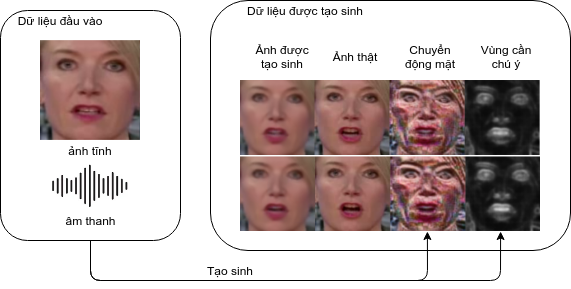
\includegraphics[width=12cm]{images/idea-small.png}
    \label{fig:idea}
    \caption{Ý tưởng tạo sinh hình ảnh từ ảnh gốc}
    \end{figure}
\end{frame}

\subsection{Cấu trúc tổng quát}

\begin{frame}{Cấu trúc tổng quát}
Hệ thống gồm có hai thành phần chính:
\begin{itemize}
    \item Mạng tạo sinh cột mốc gương mặt ($\Psi$)
    \item Hệ thống mạng GANs:
    \begin{itemize}
        \item Mạng tạo sinh video ($G$)
        \item Mạng phân biệt ($D$)
    \end{itemize}
\end{itemize}
\end{frame}

\begin{frame}{Cấu trúc tổng quát}
    \begin{figure}[H]
    \centering
    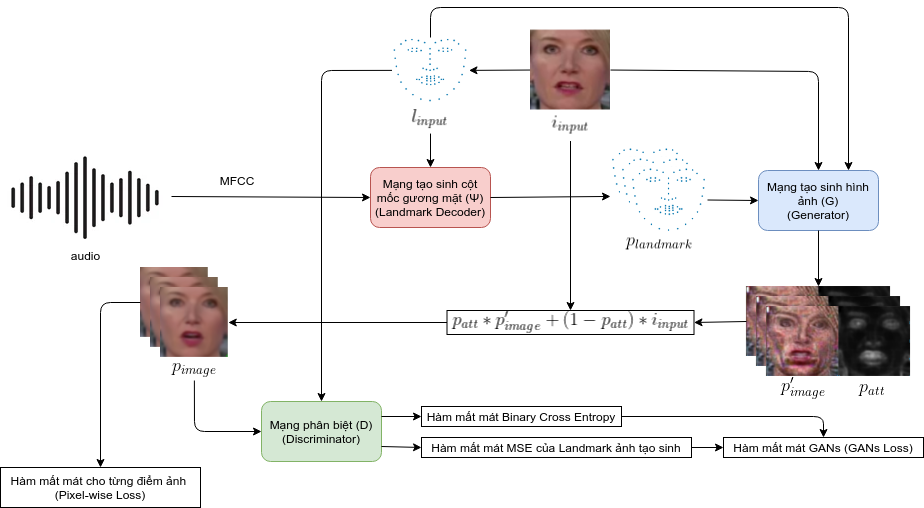
\includegraphics[width=12cm]{images/common_architecture.png}
    \label{fig:common_architecture}
    \caption{Cấu trúc tổng quát của hệ thống}
    \end{figure}
\end{frame}

\begin{frame}{Cấu trúc tổng quát}
    Hệ thống được mô hình hóa bằng công thức:
    \begin{equation}
        \begin{split}
        p_{landmark}(t) &= \Psi(l_{input}, mfcc(a(t)))\\
        p'_{image}(t), p_{att} &= G(i_{input}, l_{input}, p_{landmark})\\
        p_{image} &= p_{att}*p'_{image}+(1-p_{att})*i_{input}
        \end{split}
    \end{equation}
\end{frame}

\subsection{Tiền xử lý dữ liệu}
\begin{frame}{Tiền xử lý dữ liệu}
    Dữ liệu huấn luyện là các video với mặt người đang nói.
    \begin{itemize}
        \item Âm thanh: được trích xuất đặc trưng MFCC trước khi đưa vào mạng $\Psi$
        \item Hình ảnh: trích xuất và chuẩn hóa hình ảnh gương mặt sao cho mắt, mũi và miệng người nói trong các video có vị trí gần như nhau
        \item Cột mốc gương mặt: trích xuất và chuẩn hóa cột mốc gương mặt từ các video
    \end{itemize}
\end{frame}

\begin{frame}{Tiền xử lý dữ liệu}
    Đối với âm thanh
    \begin{figure}[H]
        \centering
        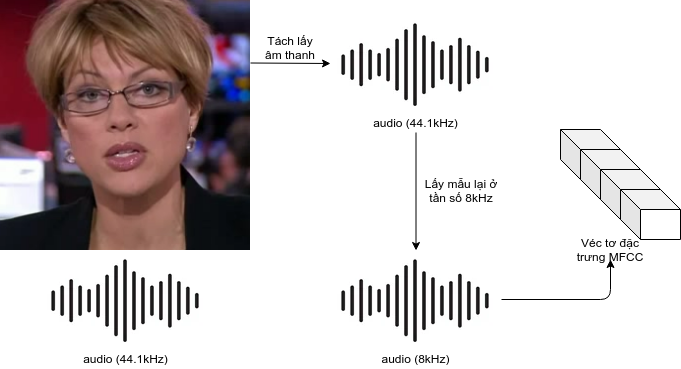
\includegraphics[width=11cm]{images/preprocess-audio.png}
        \label{fig:preprocess-audio}
        \caption{Tiền xử lý âm thanh}
    \end{figure}
\end{frame}

\begin{frame}{Tiền xử lý dữ liệu}
    Ta mong muốn đầu vào của mạng là một cột mốc gương mặt chung nhất và không bị ảnh hưởng bởi đặc điểm mặt người trên video. Vì vậy, ta cần tạo ra cột mốc gương mặt chuẩn bằng cách lấy trung bình cộng của nhiều cột mốc trong nhiều video khác nhau
    \begin{figure}[H]
        \centering
        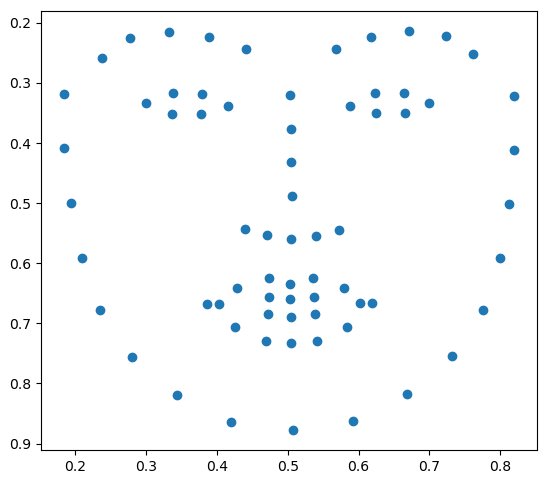
\includegraphics[width=6cm]{images/standard_landmark.png}
        \label{fig:standard_landmark}
        \caption{Cột mốc gương mặt chuẩn}
    \end{figure}
\end{frame}

\begin{frame}{Tiền xử lý dữ liệu}
    Với cách chuẩn hóa nêu trên, ta có thể đưa chuyển động của cột mốc gương mặt ban đầu lên cột mốc gương mặt chuẩn, với các góc độ quay khác nhau của video và loại bỏ đặc điểm gương mặt người nói
    \begin{figure}[H]
        \centering
        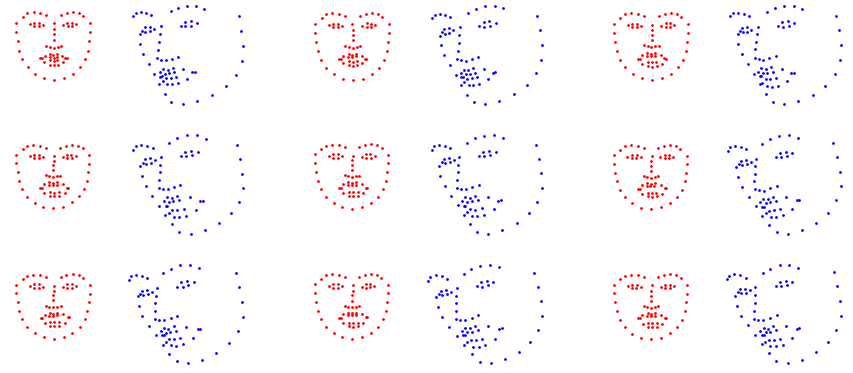
\includegraphics[width=11cm]{images/standardize_landmark.png}
        \label{fig:standardize_landmark}
        \caption{Kết quả chuẩn hóa cột mốc gương mặt. Cột mốc ban đầu (xanh), chuẩn hóa (đỏ)}
    \end{figure}
\end{frame}

\begin{frame}{Tiền xử lý dữ liệu}
    Với cách chuẩn hóa hình ảnh trên, ta có thể đưa mắt, mũi, miệng người nói trong video về một vị trí gần như nhau trong mọi video
    \begin{figure}[H]
        \centering
        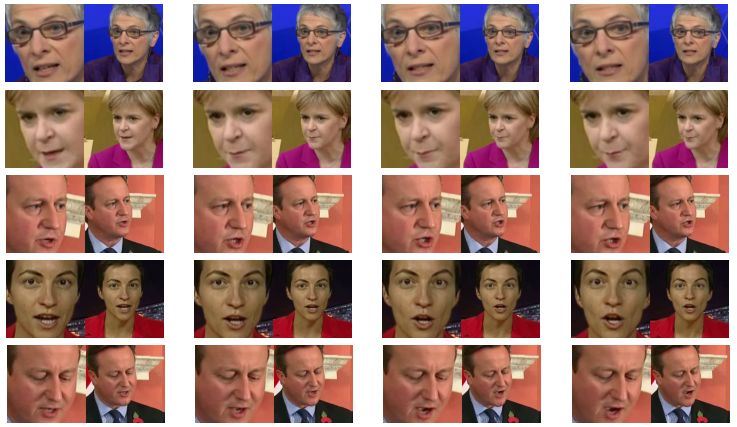
\includegraphics[width=10cm]{images/preprocess-image.png}
        \label{fig:preprocess-image}
        \caption{Kết quả chuẩn hóa hình ảnh}
    \end{figure}
\end{frame}

\subsection{Cấu trúc chi tiết}
\begin{frame}{Cấu trúc bộ giải mã cột mốc gương mặt (Landmark Decoder)}
    \begin{figure}[H]
        \centering
        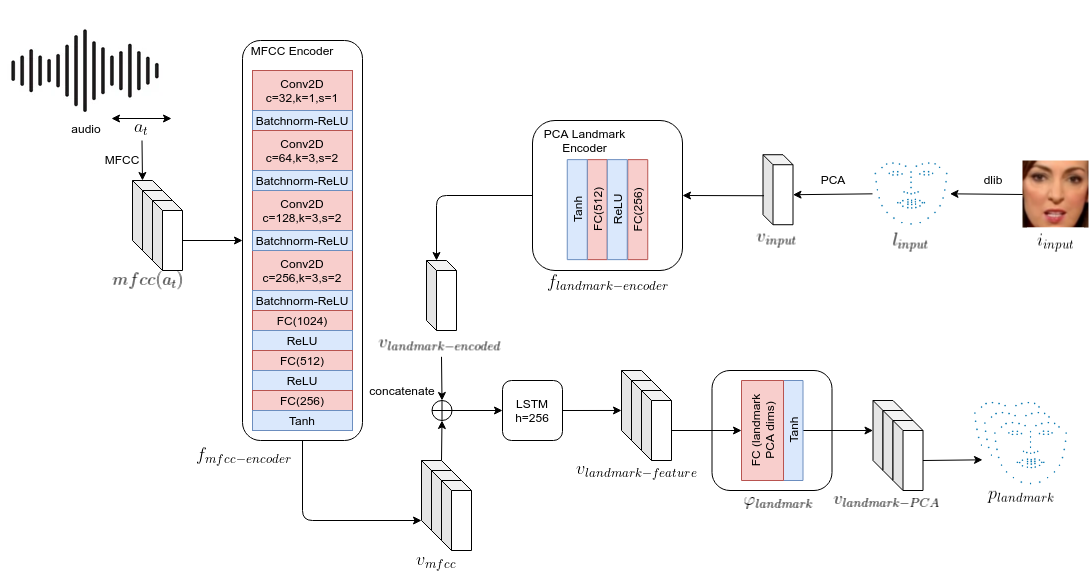
\includegraphics[width=13cm]{images/landmark_decoder.png}
        \label{fig:landmark_decoder}
        \caption{Cấu trúc bộ giải mã cột mốc gương mặt (Landmark Decoder)}
    \end{figure}
\end{frame}

\begin{frame}{Cấu trúc bộ giải mã cột mốc gương mặt (Landmark Decoder)}
    Landmark Decoder được mô hình hóa bằng công thức:
    \begin{equation}
        \begin{split}
        v_{landmark-encoded} &= f_{landmark-encoder}(PCA(l_{input}))\\
        v_{mfcc}(t) &= f_{mfcc-encoder}(mfcc(a_t))\\
        v_{landmark-feature} &= LSTM(v_{landmark-encoded} \oplus v_{mfcc})\\
        p_{landmark} &= PCA_R(\varphi_{landmark}(v_{landmark-feature}))
        \end{split}
    \end{equation}
\end{frame}

\begin{frame}{Cấu trúc bộ tạo sinh hình ảnh (Generator)}
    \begin{figure}[H]
        \centering
        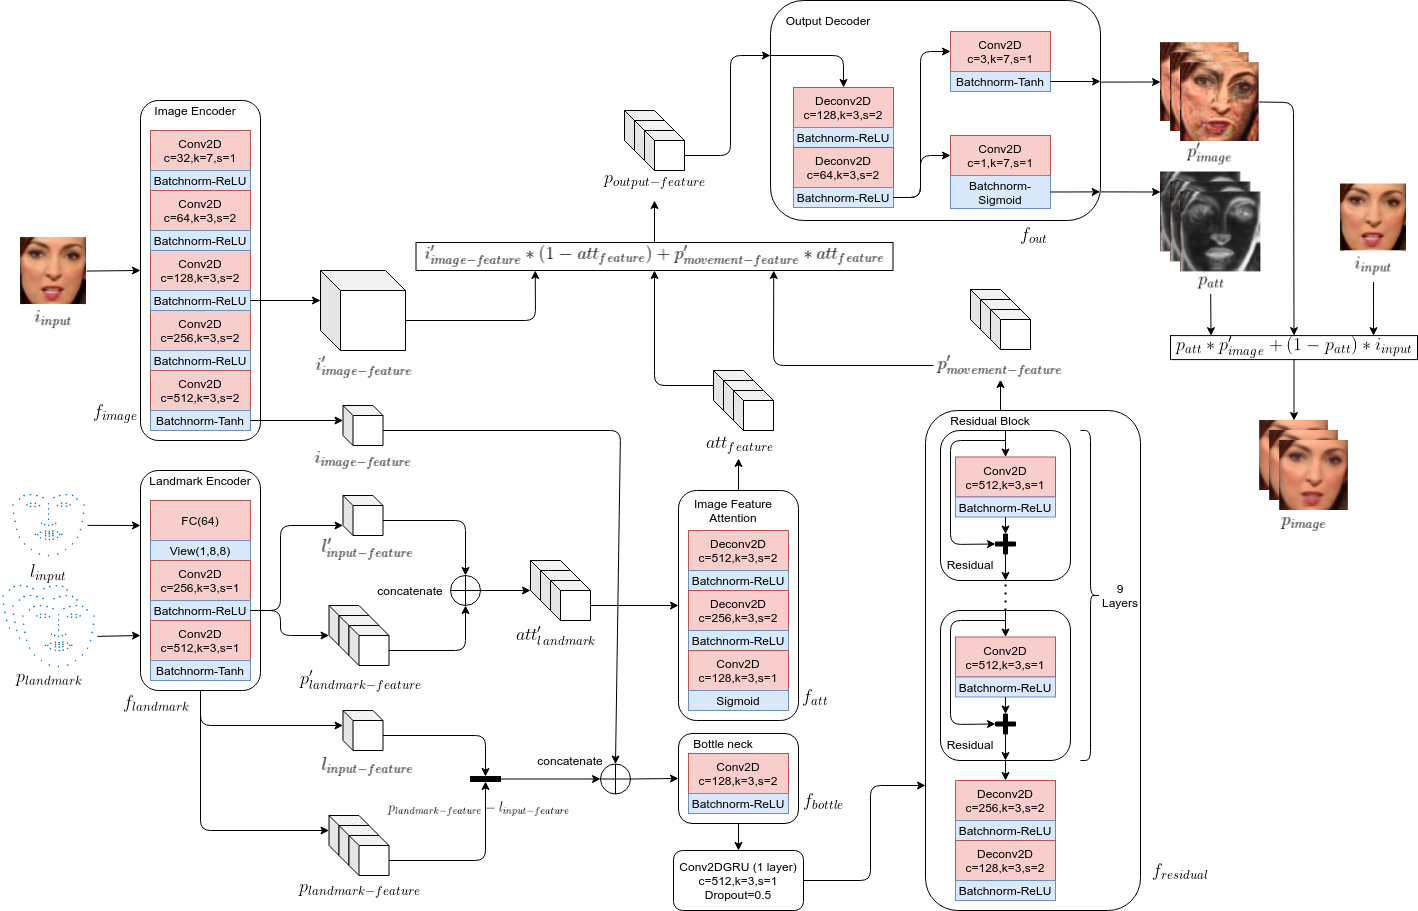
\includegraphics[width=10.5cm]{images/generator.png}
        \label{fig:generator}
        \caption{Cấu trúc bộ tạo sinh hình ảnh (Generator)}
    \end{figure}
\end{frame}

\begin{frame}{Cấu trúc bộ tạo sinh hình ảnh (Generator)}
    Generator được mô hình hóa bằng công thức:
    \begin{equation}
        \begin{split}
        i'_{image-feature}, i_{image-feature} &= f_{image}(i_{input})\\
        l'_{input-feature}, l_{input-feature} &= f_{landmark}(l_{input})\\
        p'_{landmark-feature}, p_{landmark-feature} &= f_{landmark}(p_{landmark})\\
        p'_{movement-feature}(t) &= f_{residual}(CRNN(f_{bottle}(i_{image-feature} \\
        &\oplus (p_{landmark-feature}(t)-l_{input-feature}))))\\
        att_{feature}(t) &= f_{att}(p'_{landmark-feature}(t) \oplus l'_{input-feature})\\
        p_{output-feature}(t) &= i'_{image-feature}*(1-att_{feature}(t))+\\
        &p'_{movement-feature}(t)*att_{feature}(t)\\
        p_{att}(t), p'_{image}(t) &= f_{out}(p_{output-feature}(t))\\
        p_{image}(t) &= p_{att}(t)*p'_{image}(t)+(1-p_{att}(t))*i_{image}
        \end{split}
    \end{equation}
\end{frame}

\begin{frame}{Cấu trúc bộ phân biệt (Discriminator)}
    \begin{figure}[H]
        \centering
        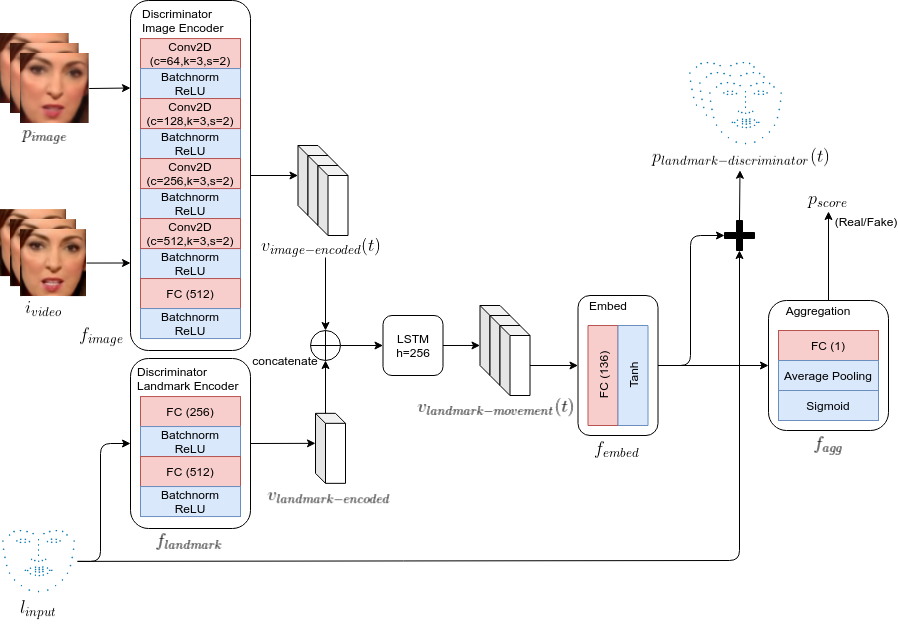
\includegraphics[width=10cm]{images/discriminator.png}
        \label{fig:discriminator}
        \caption{Cấu trúc bộ phân biệt (Discriminator)}
    \end{figure}
\end{frame}

\begin{frame}{Cấu trúc bộ phân biệt (Discriminator)}
    Discriminator được mô hình hóa bằng công thức:
    \begin{equation}
        \begin{split}
        v_{image-encoded}(t) &= f_{image}(p_{image}(t)|i_{video}(t))\\
        v_{landmark-encoded} &= f_{landmark}(l_{input})\\
        v_{landmark-movement} &= LSTM(v_{image-encoded} \oplus v_{landmark-encoded})\\
        p_{landmark-discriminator}(t) &= f_{embed}(v_{landmark-movement}(t) + l_{input})\\
        p_{score} &= f_{agg}(f_{embed}(v_{landmark-movement}))
        \end{split}
    \end{equation}
\end{frame}

\subsection{Hàm mất mát}

\begin{frame}{Hàm mất mát cho từng pixel}
    \begin{equation}
        \mathcal{L}_{pix} = \frac{1}{T}\sum^T_{t=1}||(i_{video}(t)-p_{image}(t))*(p_{att}(t)+\beta)||_1
    \end{equation}
    
    Trong đó:
    \begin{itemize}
        \item \textbf{$i_{video}(t)$}: khung hình tại thời điểm $t$ của video gốc
        \item \textbf{$p_{image}(t)$}: hình ảnh được tạo sinh tại thời điểm $t$
        \item \textbf{$p_{att}(t)$}: mặt nạ chú ý được dự đoán tại thời điểm $t$
        \item \textbf{$\beta$}: một hằng số để đảm bảo tất cả các điểm trên ảnh đều được học, ta chọn $\beta = 0.5$ 
    \end{itemize}
    
\end{frame}

\begin{frame}{Hàm mất mát GANs cho bộ phân biệt}
    \begin{equation}
        \begin{split}
        \mathcal{L}_{gans-dis} = &\mathbb{E}_{l_{input},i_{video}}[logD_s(l_{input},i_{video})]\\
        +&\mathbb{E}_{l_{input},i_{input},p_{landmark}}[log(1-D_s(l_{input},G(l_{input},i_{input},p_{landmark})))]
        \end{split}
    \end{equation}
    Trong đó:
    \begin{itemize}
        \item \textbf{$l_{input},i_{input},p_{landmark},i_{video}$}: đã được giải thích ở các phần trên
        \item \textbf{$D_s$}: Mạng phân biệt với đầu ra là xác suất ảnh là ảnh thật
        \item \textbf{$G$}: Mạng tạo sinh hình ảnh
    \end{itemize}
\end{frame}

\begin{frame}{Hàm mất mát GANs cho bộ phân biệt}
\begin{equation}
    \begin{split}
    \mathcal{L}_{gans-landmark} = &||(D_l(l_{input},G(l_{input},i_{input},p_{landmark})) - l_{orig})*M_l||^2_2\\
    +&||(D_l(l_{input},i_{video}) - l_{orig})*M_l||^2_2\\
    \end{split}
\end{equation}

    Trong đó:
    \begin{itemize}
        \item \textbf{$l_{input},i_{input},p_{landmark},i_{video}$}: đã được giải thích ở các phần trên
        \item \textbf{$D_l$}: Mạng phân biệt với đầu ra là cột mốc gương mặt trên ảnh được tạo sinh
        \item \textbf{$G$}: Mạng tạo sinh hình ảnh
        \item \textbf{$l_{original}$}: Cột mốc gương mặt được trích xuất nguyên gốc từ video $i_{video}$
        \item \textbf{$M_l$}: mặt nạ nhằm chú ý nhiều hơn vào cột mốc gương mặt vùng miệng, theo đó, sai số của cột mốc ở vùng miệng có hệ số 100, trong khi các vùng khác là 1.
    \end{itemize}
\end{frame}

\begin{frame}{Hàm mất mát tổng}
    \begin{equation}
        \begin{split}
        \mathcal{L}_{gans} = &\mathcal{L}_{gans-dis} + \mathcal{L}_{gans-landmark}\\
        \mathcal{L} = &\mathcal{L}_{gans} + \lambda*\mathcal{L}_{pix}
        \end{split}
    \end{equation}
    Với $\lambda = 10$
\end{frame}

\section{Kế hoạch nghiên cứu}\label{sec:intro}
\frame{\tableofcontents[currentsection]}
\begin{frame}{Kế hoạch nghiên cứu}

\begin{itemize}
    \item Khảo sát, thử nghiệm một số phương pháp tạo sinh ảnh dùng cơ chế attention
    \item Khảo sát, thử nghiệm thêm một số phương pháp tạo sinh ảnh sử dụng các đặc trưng trong không gian ba chiều.
    \item Tiến hành thiết, hiện thực và kiểm chứng các kiến trúc mạng mới dựa trên những kiến thức đã thu thập được.
    \item Tổng hợp các thử nghiệm và lựa chọn kiến trúc mạng tốt nhất cho Luận văn.
    \item Viết báo cáo và bảo vệ Luận văn.
\end{itemize}
\end{frame}

\section{Kết quả dự kiến}\label{sec:intro}
\frame{\tableofcontents[currentsection]}
\begin{frame}{Kết quả dự kiến}

\begin{itemize}
    \item Xây dựng được mô hình tính toán mới, có khả năng tạo sinh hình ảnh mặt người một cách chân thật.
    \item Luận văn cũng sẽ cung cấp được các đánh giá và so sánh khách quan với các mô hình hiện tại bằng số liệu thực tế.
\end{itemize}
\end{frame}


\bibliographystyle{unsrt}
\bibliography{references}
\include{./references}



\begin{frame}
    \textbf{\LARGE{\begin{center}Thank you for your attention\end{center}}}
\end{frame}

\end{document}
